\subsection{Optimization Attempts of Branch Target Buffer}

In this subsection, we present our optimization strategies and experimental results for improving the performance of the Branch Target Buffer (BTB). We evaluated several aspects including BTB size, associativity, eviction policies, warm-up strategies, and integration with branch history. Our goal was to reduce the BTB miss rate and, consequently, improve the overall CPI (Cycles Per Instruction) of the program. The following tests are all done on short programs.

\subsubsection{Miss Rate Calculation}

The BTB miss rate is defined as the ratio of missed conditional and taken branches to the total number of conditional branches. Formally, we compute:

\[
\text{Miss Rate} = \frac{\#(\text{missed} \land \text{taken} \land \text{conditional})}{\#(\text{conditional branches})}
\]

This metric directly influences the control hazard penalty, making it a crucial indicator of BTB effectiveness.

\subsubsection{Direct-Mapped BTB Performance with Varying Sizes}

We first explored how increasing the size of a direct-mapped BTB affects performance. The miss rate decreases significantly as we increase the number of entries, but the improvement plateaus after a certain threshold due to diminishing returns. Below is a plot (omitted in this snippet) that shows this trend.

\begin{center}
\begin{tabular}{|c|c|}
\hline
\textbf{BTB Size (entries)} & \textbf{Miss Rate} \\
\hline
16 & 0.2529 \\
32 & 0.1876 \\
64 & 0.0867 \\
128 & 0.0820 \\
\hline
\end{tabular}
\end{center}

We observed a large performance gain up to 32 entries. Beyond that, the gain becomes marginal, suggesting 32 as a good trade-off point between performance and storage.
\begin{figure}[htbp]
    \centering
    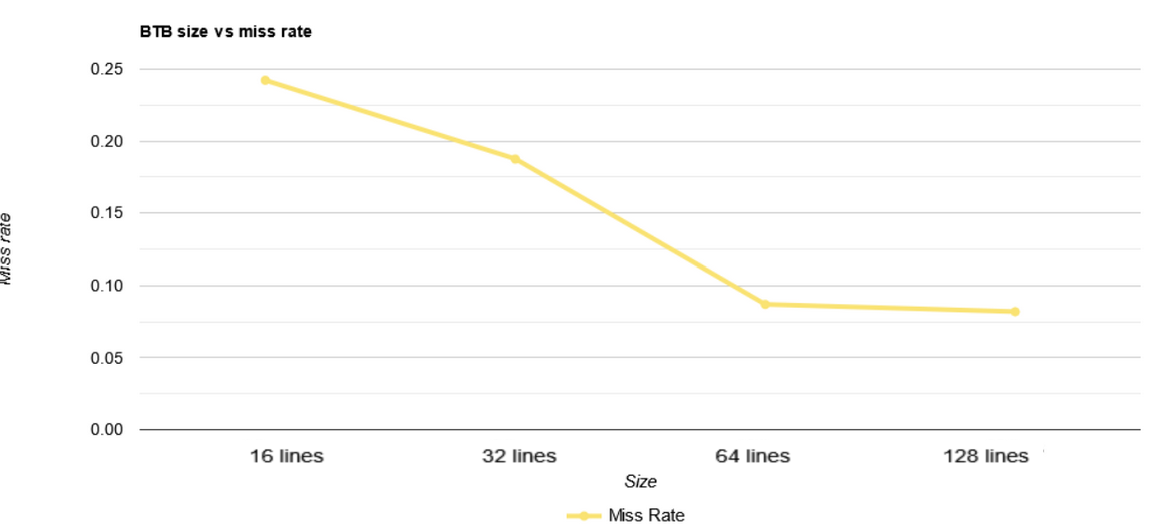
\includegraphics[width=0.5\textwidth]{figures/btb_missrate.png} % Replace with your image filename
    \caption{Relationship between btb size and miss rate on short programs.}
    \label{fig:sample-figure}
\end{figure}

\subsubsection{Direct-Mapped vs 4-Way Set Associative BTB}

Next, we compared a direct-mapped(DM) BTB and a 4-way set-associative(4-way SA) BTB, ensuring both have the same total number of entries (32). The associative BTB significantly reduces miss rate by mitigating conflicts.

\begin{center}
\textit{NM: Normalized}
\par\medskip
\begin{tabular}{|c|c|}
\hline
\textbf{BTB Configuration} & \textbf{Miss Rate}  \\
\hline
DM (32 lines) & 0.1876  \\
4-Way SA (8 sets) & 0.0686  \\
\hline
\end{tabular}
\end{center}

However, there is no significant CPI improvement on short programs, except for sort\_search.c.
\subsubsection{Round-Robin vs LRU Eviction Policies}

For set-associative BTBs, we explored two eviction strategies: Round-Robin and Least Recently Used (LRU). The main difference lies in whether the "used" bit is updated upon access.

\begin{center}
\begin{tabular}{|c|c|}
\hline
\textbf{Eviction Policy} & \textbf{Miss Rate} \\
\hline
Round-Robin & 0.0687  \\
LRU & 0.0686 \\
\hline
\end{tabular}
\end{center}

The results suggest that while LRU slightly outperforms Round-Robin, the difference is negligible in practice, especially considering the added complexity of tracking LRU.

\subsubsection{Hot Loading (Warm-Up Phase)}

Inspired by the idea of branch prediction warm-up, we implemented a "hot loading" strategy. We first ran the program once to collect BTB entries and then constructed a synthetic BTB to preload during program startup. This method aims to approximate a well-warmed-up BTB from the beginning of execution.

\begin{center}
\begin{tabular}{|c|c|}
\hline
\textbf{BTB State} & \textbf{Miss Rate} \\
\hline
No Warm-Up & 0.0686 \\
Hot-Loaded BTB & 0.0647 \\
\hline
\end{tabular}
\end{center}

This approach yielded a small yet consistent improvement, especially in short-running programs where warm-up matters more.

\subsubsection{Integration with Branch History}

To address the issue where the same branch address may lead to different targets (e.g., due to function pointers), we experimented with augmenting the BTB with branch history. We used both 2-bit and 3-bit global history mechanisms, applied to direct-mapped BTBs.

\begin{center}
\begin{tabular}{|c|c|}
\hline
\textbf{BTB Configuration} & \textbf{Miss Rate} \\
\hline
Direct-Mapped Only & 0.1876 \\
Direct-Mapped + 2-bit History & 0.1878 \\
Direct-Mapped + 3-bit History & 0.1924 \\
\hline
\end{tabular}
\end{center}

Unfortunately, incorporating short branch histories did not yield performance gains in our setup. We suspect that the history length was insufficient to capture meaningful patterns or that target aliasing was minimal in our benchmarks.

